%%%%%%%%%%%%%%%%%%%%%%%%%%%%%%%%%%%%%%%%%
%
% Reproducible Research Workshop Slides
% Module 04
% Perry Williams
% 09/12/2020
%
%%%%%%%%%%%%%%%%%%%%%%%%%%%%%%%%%%%%%%%%%

% ---------------------------------------------------------
%	PACKAGES AND THEMES
% ---------------------------------------------------------

\documentclass{beamer}\usepackage[]{graphicx}\usepackage[]{color}
%% maxwidth is the original width if it is less than linewidth
%% otherwise use linewidth (to make sure the graphics do not exceed the margin)
\makeatletter
\def\maxwidth{ %
  \ifdim\Gin@nat@width>\linewidth
    \linewidth
  \else
    \Gin@nat@width
  \fi
}
\makeatother

\usepackage{Sweavel}



\usetheme{Madrid}
\usecolortheme{beaver}

\setbeamertemplate{navigation symbols}{}
\setbeamercolor{block title}{fg=black,bg=darkred}
\setbeamercolor{block body}{fg=black,bg=lightgray}


\usepackage{animate}
\usepackage{booktabs}
\usepackage{graphicx}
\usepackage{mathtools}
\usepackage{mathrsfs}
\usepackage{media9}
\usepackage{listings}
\usepackage{pgf}
\usepackage{stackengine}
\usepackage{textpos}
\usepackage{tikz}
\usepackage{xcolor}
\lstset{breaklines=true} % break long lines
\newcommand\Fontvi{\fontsize{14}{7.2}\selectfont}
\newcommand{\backupbegin}{
  \newcounter{finalframe}
  \setcounter{finalframe}{\value{framenumber}}
}
\newcommand{\backupend}{
  \setcounter{framenumber}{\value{finalframe}}
}
\renewcommand\useanchorwidth{T}
\def\theyearwidth{1.5pt}
\newlength\yrsfboxrule
\yrsfboxrule .4\fboxrule
\newcommand\yearwidth[1]{\def\theyearwidth{#1}\ignorespaces}
\newcommand\skipyears[2][white]{%
  \fboxrule\yrsfboxrule%
  \fboxsep=-\yrsfboxrule%
  \fcolorbox{gray}{#1}{\strut\hspace{#2}}%
  \ignorespaces%
}
\newcommand\showyear[2][black]{%
  \fboxsep=0pt%
  \stackon{%
    \colorbox{#1}{\strut\hspace{\theyearwidth}}
  }{\sffamily\small#2}%
  \ignorespaces%
}

\let\svthefootnote\thefootnote
\textheight 1in
\newcommand\blankfootnote[1]{%
  \let\thefootnote\relax\footnotetext{#1}%
  \let\thefootnote\svthefootnote%
}
\usetikzlibrary{fadings}
\tikzfading[name=fade out, inner color=transparent!0,
         outer color=transparent!100]

\graphicspath{{./Images/}}

% ---------------------------------------------------------
%	TITLE PAGE
% ---------------------------------------------------------

\title[Reproducible Research]{\normalsize GRAD 778: Reproducible Research}
\author[Perry Williams]{\footnotesize Perry J. Williams}
\vspace{1in}
\institute[]{
  Department of Natural Resources and Environmental Science\\
  University of Nevada, Reno}
\date[\today]{\today}
\begin{document}

\begin{frame}
\begin{textblock*}{4cm}(8cm,5.8cm) % {block width} (coords)
      \begin{tikzpicture} \path (0,0) rectangle
        (5,7); \node[scope fading=fade out,inner
        sep=0pt,outer sep=0pt,anchor=south east]
        at(5,5)
        {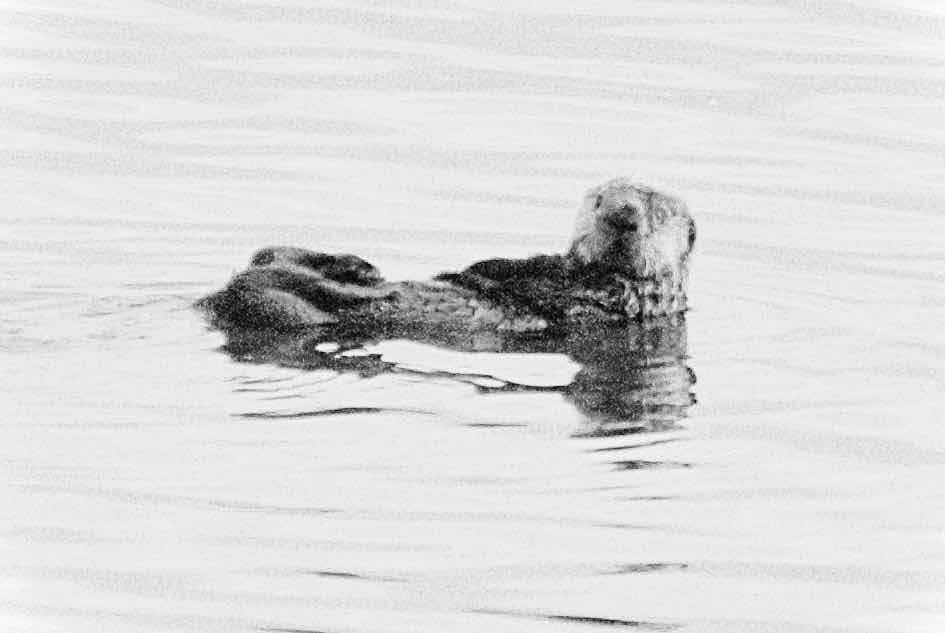
\includegraphics[width=5cm]{icon2}};
      \end{tikzpicture}
  \end{textblock*}
\begin{textblock*}{4cm}(-2cm,5.5cm) % {block width} (coords)
      \begin{tikzpicture} \path (0,0) rectangle
        (5,7); \node[scope fading=fade out,inner
        sep=0pt,outer sep=0pt,anchor=south east]
        at(5,5)
        {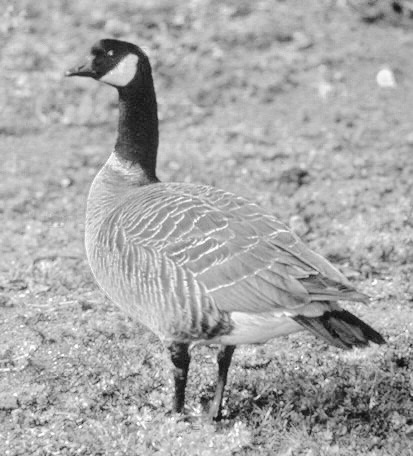
\includegraphics[width=3cm]{cago3}};
      \end{tikzpicture}
  \end{textblock*}
  \titlepage
\end{frame}

% -------------------------------------------------------
% PRESENTATION SLIDES
% -------------------------------------------------------



% ------------------------------------------------
\section{Background \& Motivation}
% ------------------------------------------------

\begin{frame}[noframenumbering]
  \begin{center}
      \textsc{\textrm{Background \& Motivation}}
  \end{center}
\end{frame}


\begin{frame}{Background \& Motivation}
  \begin{center}
    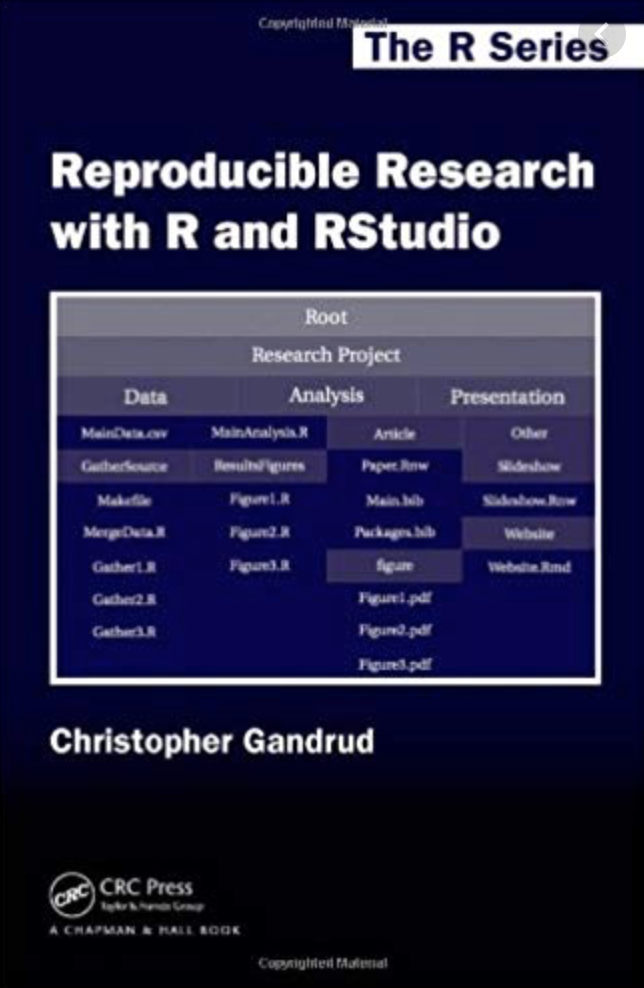
\includegraphics[height=\textheight,keepaspectratio]{rr}
  \end{center}
\end{frame}

\begin{frame}[t]{Background \& Motivation}
  \textbf{Research is often presented in very abridged packages}
    \begin{itemize}
      \item Slide shows
      \item Journal articles
      \item Books
      \item Web sites
    \end{itemize}
\end{frame}

\begin{frame}[t]{Background \& Motivation}
  \textbf{These presentation documents announce a project's findings}
\end{frame}

\begin{frame}[t]{Background \& Motivation}
  \textbf{These documents are not the research}
  \begin{itemize}
 \item These documents are the advertising
  \item Especially true in computational and statistical sciences
  \end{itemize}
\end{frame}

\begin{frame}[t]{Background \& Motivation}
  \textbf{The research includes:}
  \begin{itemize}
    \item Full software environment
    \item Code
    \item Data
  \end{itemize}
\end{frame}

\begin{frame}[t]{Background \& Motivation}
  \textbf{When we separate the research from its advertisement we make it difficult for other to reproduce our findings}
\begin{center}
    
\includegraphics[height=0.8\textheight,keepaspectratio]{finaldoc}
  \end{center}
\end{frame}

\begin{frame}[t]{Background \& Motivation}
   \textbf{This workshop will introduce:}
   \begin{itemize}
\item  The tools to dynamically combine research with presentation of findings,
     \item The \textbf{\texttt{R}} statistical language for data analysis,
     \item the \textbf{\LaTeX} mark-up language for documents, slide shows, articles, books, and web-pages,
     \item the \texttt{knitr} package for \texttt{R},
     \item \textbf{RStudio}, a program that brings all of these tools together in one place.
   \end{itemize}
 \end{frame}

 \begin{frame}[t]{Objective}
   \textbf{The objective of this workshop is to:}
   \begin{itemize}
      \item   Introduce the tools to develop a work-flow to maximize reproducible-ness, collaborations, and research impact.
      \item Provide templates that can be modified for your own research.
   \end{itemize}
   \textbf{The objective of this workshop is not to:}
   \begin{itemize}
      \item Become well-versed in \texttt{R}, \texttt{RStudio}, \texttt{\LaTeX}, or \texttt{knitr} - that takes repetition (starting with the basic building blocks that are provided).
   \end{itemize}
\end{frame}
 
\begin{frame}[t]{Background \& Motivation}
   \textbf{Additional topics include:}
   \begin{itemize}
\item  Version control with Git hub,
     \item Data gathering,
     \item R markdown,
     \item File management,
     \item Projects in RStudio,
     \item Using \LaTeX to make presentations with Beamer. 
   \end{itemize}
   \textbf{All are covered in the book:} \emph{Reproducible Research with R and RStudio}
\end{frame}

 \begin{frame}[t]{Why \texttt{R}?}
  \begin{itemize}
    \item Open Source and free
    \item Very active development community
    \item Interfaces with \LaTeX or other mark-up languages
    \item Explicitly write down analyses steps as source code
   \end{itemize}
 \end{frame}

 \begin{frame}[t]{Why \texttt{knitr}?}
  \begin{itemize}
    \item Literate programming is a crucial part of reproducible quantitative research
    \item Highlights \texttt{R} code in presentation documents making it easier for readers to follow
    \item Provides control over inclusion of graphics
    \item Can cache (save output for later)
   \end{itemize}
 \end{frame}

 \begin{frame}[t]{Why RStudio?}
  \begin{itemize}
    \item Stand alone editor for \TeX  and Markdown
    \item Many shortcuts
    \item Works with C++, CSS, JavaScript, and a few other programming languages
    \item Integrated with version control of Git and SVN
    \item Simple compiling of .Rnw files
    \item \textbf{Easier to learn than Emacs or vi!}
   \end{itemize}
 \end{frame}

% ------------------------------------------------
\section{What is Reproducible Research?}
% ------------------------------------------------

\begin{frame}[t]{What is Reproducible Research?}
     Research results are replicable if there is sufficient information available for independent researchers to make the same findings using the same procedures (King, 1995, 444). \\ \vspace{2cm}
  \only<2->{\textbf{In computational sciences, this means:} \\
  The data and code used to make a finding are available and they are sufficient for an independent researcher to recreate the finding.}
  \end{frame}

% ------------------------------------------------
\section{Getting Started with R}
% ------------------------------------------------

\begin{frame}[noframenumbering]
  \begin{center}
      \textsc{\textrm{Getting Started with R}}
  \end{center}
\end{frame}

\begin{frame}{Using R: the Basics}
  \begin{itemize}
    \item objects \& assignment,
    \item component selection,
    \item functions and commands,
    \item arguments,
    \item the workspace,
    \item packages.
  \end{itemize}
\end{frame}

\begin{frame}{Objects \& Assignment}
  \begin{itemize}
    \item \texttt{R} is an ``object-oriented language''
    \item Objects are analogous to nouns
    \item ``object-oriented:'' \texttt{R} is focused on
      doing actions to objects
  \end{itemize}
\end{frame}

\begin{frame}[fragile]{Create Objects}
\begin{Schunk}
\begin{Sinput}
Number=10
\end{Sinput}
\end{Schunk}
To see the contents of our object, type its name.

\begin{Schunk}
\begin{Sinput}
Number
\end{Sinput}
\begin{Soutput}
[1] 10
\end{Soutput}
\end{Schunk}
\end{frame}

\begin{frame}[fragile]{Create Objects}
  \textbf{Create a character string}
\begin{Schunk}
\begin{Sinput}
Words="Hello World!"
\end{Sinput}
\end{Schunk}
To see the contents of our object, type its name.
\begin{Schunk}
\begin{Sinput}
Words
\end{Sinput}
\begin{Soutput}
[1] "Hello World!"
\end{Soutput}
\end{Schunk}
\end{frame}

\begin{frame}[fragile]{Vectors}
  \textbf{Create a numeric vector called} \texttt{foo}
\begin{Schunk}
\begin{Sinput}
foo=c(2,4,6,8,10,12,14,16,18)
\end{Sinput}
\end{Schunk}
To see the contents of our object, type its name.
\begin{Schunk}
\begin{Sinput}
foo
\end{Sinput}
\begin{Soutput}
[1]  2  4  6  8 10 12 14 16 18
\end{Soutput}
\end{Schunk}
\end{frame}

\begin{frame}[fragile]{Vectors}
  \textbf{Create a vector of strings called} \texttt{bar}
\begin{Schunk}
\begin{Sinput}
bar=c("the","quick", "brown","fox", "jumps",
"over","the","lazy","dog")
\end{Sinput}
\end{Schunk}
To see the contents of our object, type its name.
\begin{Schunk}
\begin{Sinput}
print(bar)
\end{Sinput}
\begin{Soutput}
[1] "the"   "quick" "brown" "fox"   "jumps" "over"  "the"   "lazy"  "dog"  
\end{Soutput}
\end{Schunk}
\end{frame}

\begin{frame}[fragile]{Matrices}
  \textbf{Create a $9\times 2$ matrix called \texttt{baz.m} using \texttt{foo} and \texttt{bar}}
\begin{Schunk}
\begin{Sinput}
baz.m=cbind(foo,bar)
\end{Sinput}
\end{Schunk}
To see the contents of our object, type its name.
\begin{Schunk}
\begin{Sinput}
print(baz.m)
\end{Sinput}
\begin{Soutput}
      foo  bar    
 [1,] "2"  "the"  
 [2,] "4"  "quick"
 [3,] "6"  "brown"
 [4,] "8"  "fox"  
 [5,] "10" "jumps"
 [6,] "12" "over" 
 [7,] "14" "the"  
 [8,] "16" "lazy" 
 [9,] "18" "dog"  
\end{Soutput}
\end{Schunk}
\end{frame}

\begin{frame}[fragile]{Data frames}
  \textbf{Create a $9\times 2$ data frame called \texttt{baz.df} using \texttt{foo} and \texttt{bar}}
\begin{Schunk}
\begin{Sinput}
baz.df=data.frame(foo,bar)
\end{Sinput}
\end{Schunk}
To see the contents of our object, type its name.
\begin{Schunk}
\begin{Sinput}
print(baz.df)
\end{Sinput}
\begin{Soutput}
  foo   bar
1   2   the
2   4 quick
3   6 brown
4   8   fox
5  10 jumps
6  12  over
7  14   the
8  16  lazy
9  18   dog
\end{Soutput}
\begin{Sinput}
names(baz.df)
\end{Sinput}
\begin{Soutput}
[1] "foo" "bar"
\end{Soutput}
\end{Schunk}
\end{frame}

\begin{frame}[fragile]{Data frames}
  \textbf{Assign row names}
\begin{Schunk}
\begin{Sinput}
row.names(baz.df)=c("Row1","Row2","Row3","Row4","Row5",
                    "Row6","Row7","Row8","Row9")
row.names(baz.df)
\end{Sinput}
\begin{Soutput}
[1] "Row1" "Row2" "Row3" "Row4" "Row5" "Row6" "Row7" "Row8" "Row9"
\end{Soutput}
\end{Schunk}
\end{frame}

\begin{frame}[fragile]{Component Selection: Sub-scripts}
  \textbf{Select rows 3--7 from baz.df}
\begin{Schunk}
\begin{Sinput}
baz.df[3:7,]
\end{Sinput}
\begin{Soutput}
     foo   bar
Row3   6 brown
Row4   8   fox
Row5  10 jumps
Row6  12  over
Row7  14   the
\end{Soutput}
\end{Schunk}
\textbf{Select rows 3--7 and column 2 from baz.df}
\begin{Schunk}
\begin{Sinput}
baz.df[3:7,2]
\end{Sinput}
\begin{Soutput}
[1] brown fox   jumps over  the  
Levels: brown dog fox jumps lazy over quick the
\end{Soutput}
\begin{Sinput}
 is.factor(baz.df[3:7,2])
\end{Sinput}
\begin{Soutput}
[1] TRUE
\end{Soutput}
\end{Schunk}
\end{frame}


\begin{frame}[fragile]{Functions and Commands}
   \textbf{If objects are the nouns, functions and commands are the verbs}
\begin{Schunk}
\begin{Sinput}
mean(baz.df[,1])
\end{Sinput}
\begin{Soutput}
[1] 10
\end{Soutput}
\begin{Sinput}
mean(baz.df[2:7,1])
\end{Sinput}
\begin{Soutput}
[1] 9
\end{Soutput}
\begin{Sinput}
?mean
\end{Sinput}
\end{Schunk}
\end{frame}

\begin{frame}[fragile]{The workspace}
   \textbf{Use the \texttt{ls()} command to list all objects in your
     current workspace}
\begin{Schunk}
\begin{Sinput}
ls()
\end{Sinput}
\begin{Soutput}
[1] "bar"    "baz.df" "baz.m"  "foo"    "Number" "Words" 
\end{Soutput}
\end{Schunk}
\end{frame}

\begin{frame}[fragile]{The workspace}
  \textbf{Use the \texttt{rm()} command to remove objects in your current workspace}
\begin{Schunk}
\begin{Sinput}
rm(baz.m)
\end{Sinput}
\end{Schunk}
\end{frame}

\begin{frame}[fragile]{Save the workspace}
   \textbf{Use the \texttt{save.image()} command to save your current workspace}
\begin{Schunk}
\begin{Sinput}
save.image(file="ShortCourseWorkspace.RData")
\end{Sinput}
\end{Schunk}
\end{frame}

\begin{frame}[fragile]{Clear the workspace}
  \textbf{Use the \texttt{rm(list=ls())} command to remove ALL objects in your current workspace}
\begin{Schunk}
\begin{Sinput}
rm(list=ls())
\end{Sinput}
\end{Schunk}
\end{frame}

\begin{frame}[fragile]{Load the workspace}
   \textbf{Use the \texttt{load()} command to load your
     saved workspace}
\begin{Schunk}
\begin{Sinput}
load(file="ShortCourseWorkspace.RData")
ls()
\end{Sinput}
\begin{Soutput}
[1] "bar"    "baz.df" "foo"    "Number" "Words" 
\end{Soutput}
\end{Schunk}
\end{frame}

\begin{frame}[fragile]{Save a specific object}
  \textbf{Use the \texttt{save()} command to save an object that was computationally intensive}
\begin{Schunk}
\begin{Sinput}
tock=Sys.time()
nr=2000
nc=2000
n=nr*nc
foo.m=matrix(rnorm(n),nr,nc)
bar.m=solve(foo.m)  # O(n^3) complexity
tick=Sys.time()
tick-tock
\end{Sinput}
\begin{Soutput}
Time difference of 7.161771 secs
\end{Soutput}
\begin{Sinput}
save(bar.m,file="MatrixInverse.RData")
rm(bar.m)
load(file="MatrixInverse.RData")
ls()
\end{Sinput}
\begin{Soutput}
 [1] "bar"    "bar.m"  "baz.df" "foo"    "foo.m"  "n"      "nc"    
 [8] "nr"     "Number" "tick"   "tock"   "Words" 
\end{Soutput}
\end{Schunk}
\end{frame}

\begin{frame}[fragile]{Packages}
\begin{Schunk}
\begin{Sinput}
install.packages("Matrix",repos='http://cran.us.r-project.org')
\end{Sinput}
\begin{Soutput}

The downloaded binary packages are in
	/var/folders/2s/9zz_mdbn2652586wqzndfp200000gn/T//RtmpUBsElX/downloaded_packages
\end{Soutput}
\begin{Sinput}
library(Matrix)
\end{Sinput}
\end{Schunk}
\end{frame}

% ------------------------------------------------
\section{Using RStudio}
% ------------------------------------------------

\begin{frame}[noframenumbering]
  \begin{center}
      \textsc{\textrm{Using RStudio}}
  \end{center}
\end{frame}

\begin{frame}
  \begin{center}
    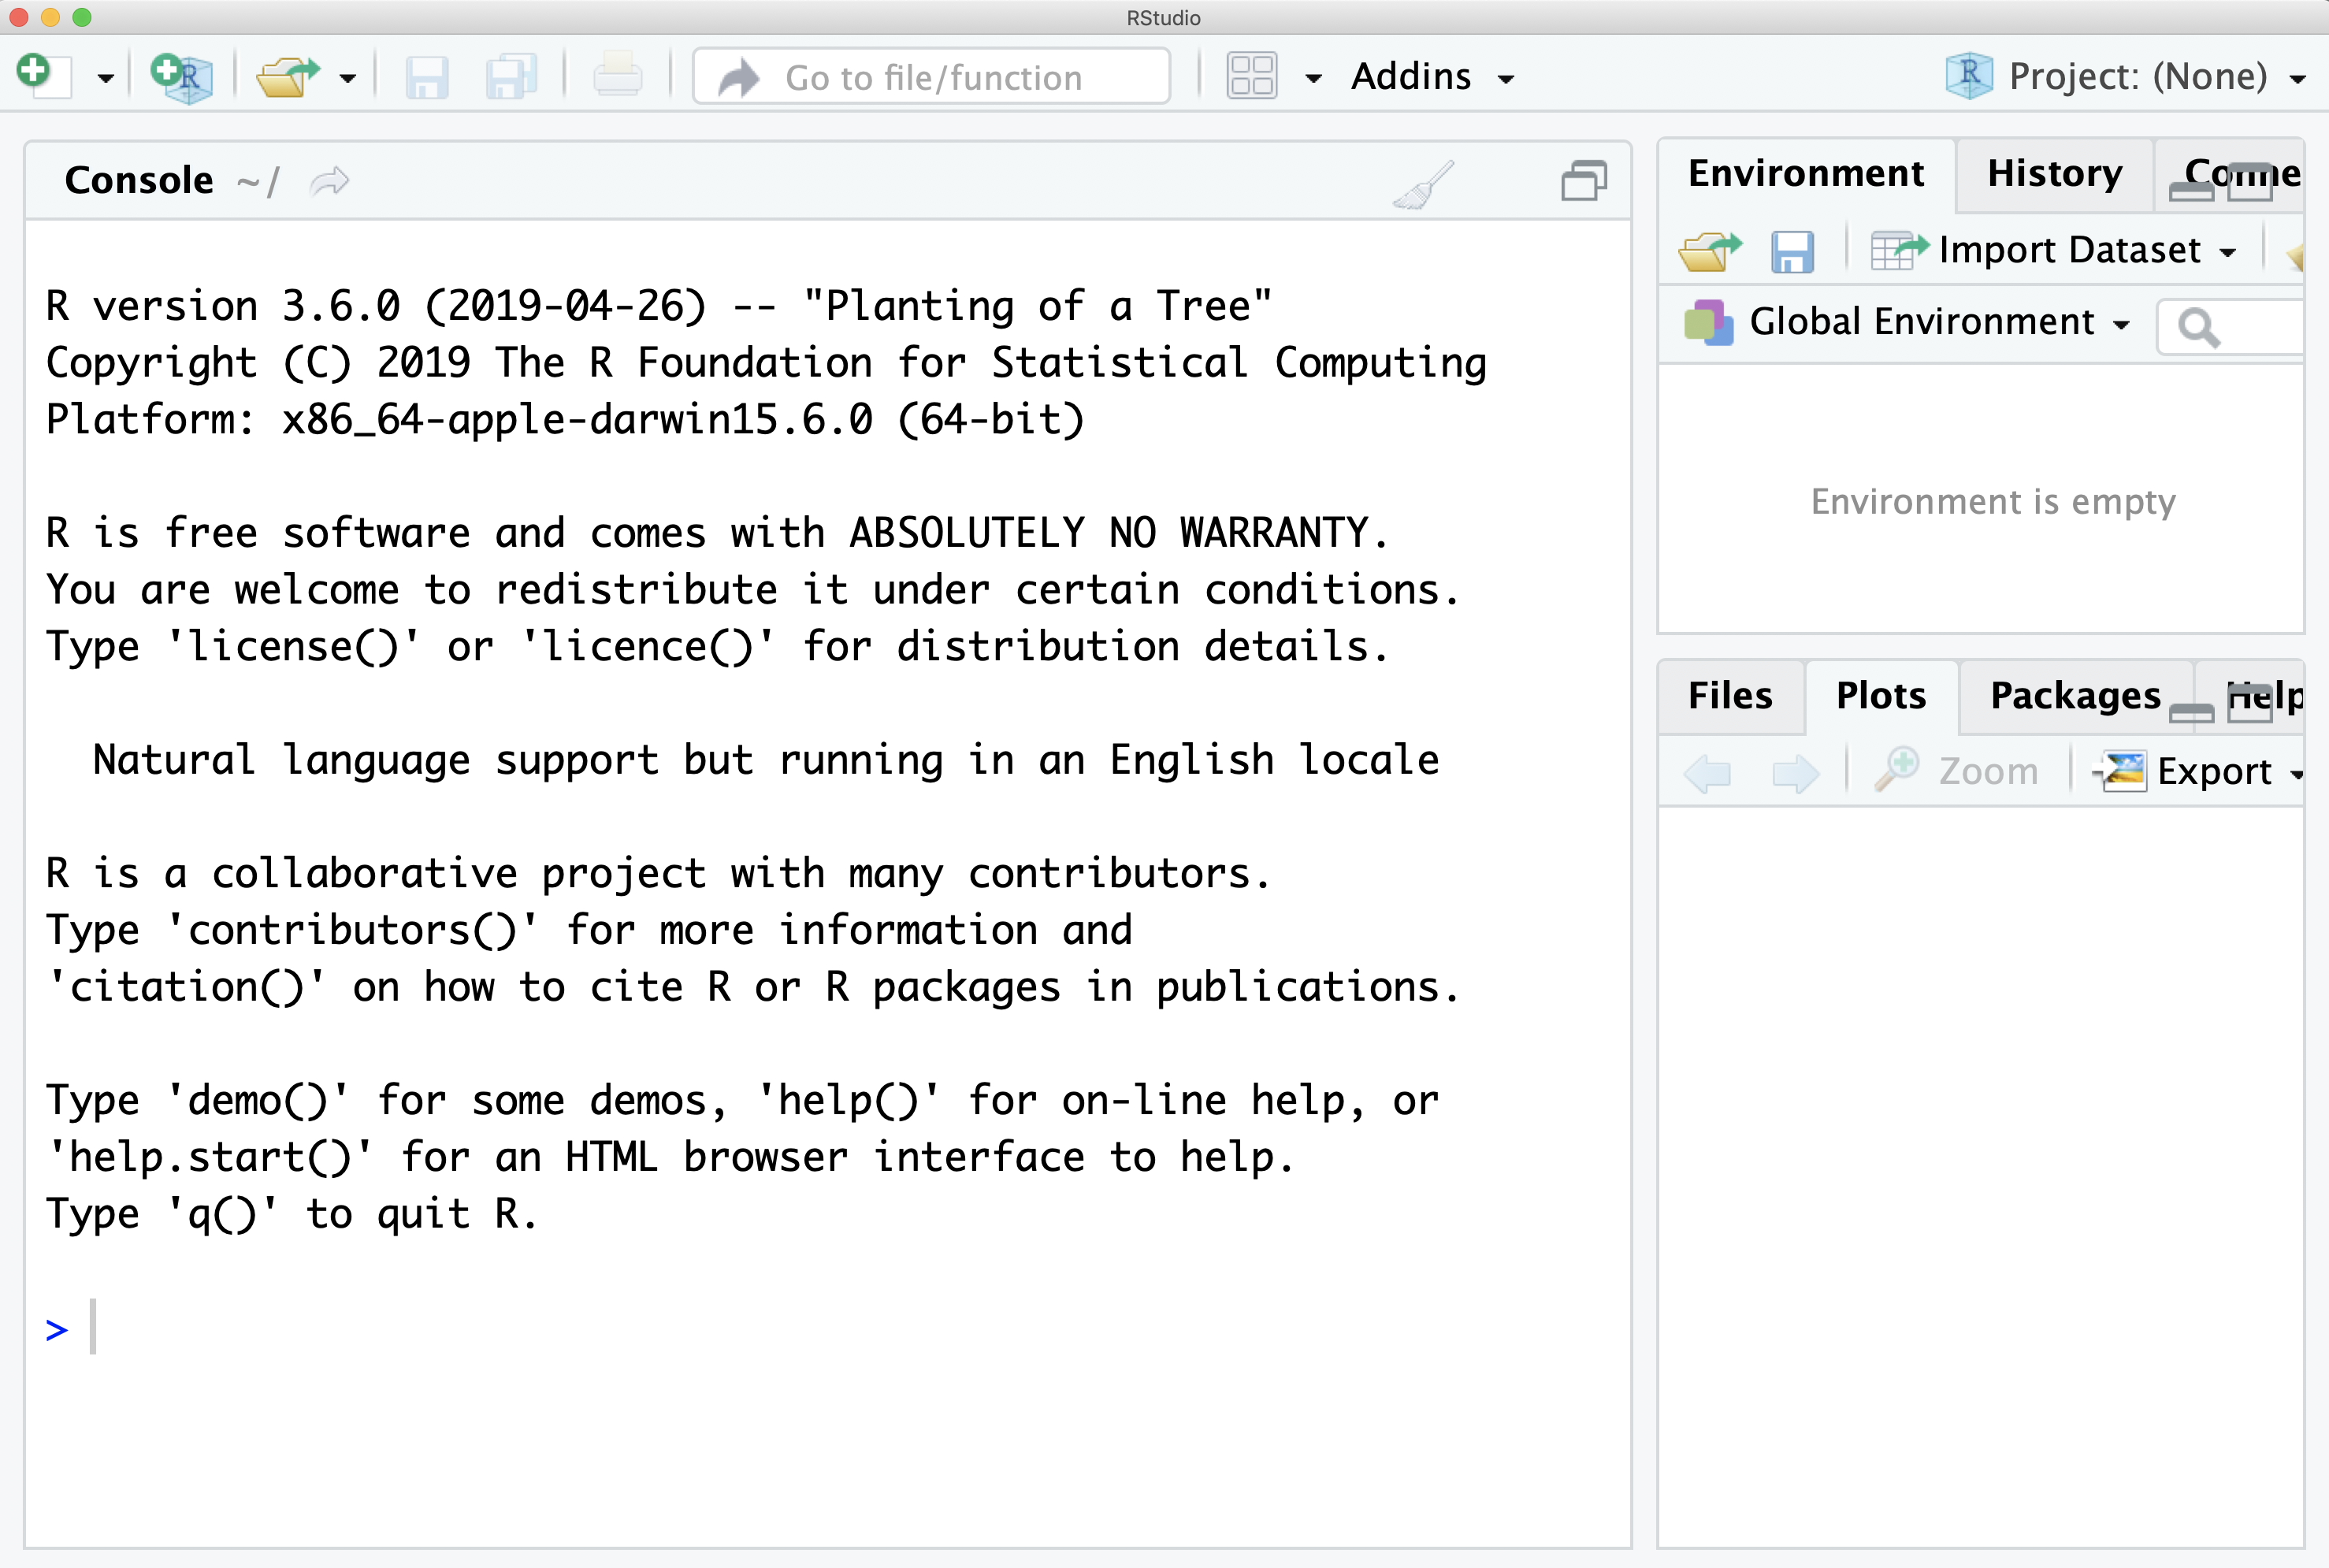
\includegraphics[width=.9\linewidth]{rstudio}
  \end{center}
\end{frame}

% ------------------------------------------------
\section{Using \LaTeX}
% ------------------------------------------------


\begin{frame}[noframenumbering]
  \begin{center}
      \textsc{\textrm{Using \LaTeX}}

   \end{center}
\end{frame}

\begin{frame}{Basic \LaTeX command syntax}
  \begin{itemize}
  \item Latex command begin with a backslash
  \item The arguments for Latex commands are written inside of curly braces
  \end{itemize}
\end{frame}


\begin{frame}[fragile]
  \begin{lstlisting}
    \documentclass{article}


     \title{My First \LaTeX Document}
     \author{Jane Doe}
     \date{\today}

     \begin{document}
     \maketitle
     Hello world!
     \end{document}

\end{lstlisting}
\end{frame}

\begin{frame}
  \begin{center}
    
\includegraphics[width=.8\linewidth,keepaspectratio]{latex1}
  \end{center}
\end{frame}


\begin{frame}[fragile]
  \tiny
  \begin{lstlisting}
    \documentclass{article}

    \usepackage{lipsum}

    \title{My Second \LaTeX Document}
    \author{Jane Doe}
    \date{September 2019}

    \begin{document}
    \maketitle
    \section{Abstract}
    \lipsum[2-4]

    \section{Introduction}
    \lipsum[2-4]

    \section{Methods}
    \lipsum[2-4]

    \section{Results}
    \lipsum[2-4]

    \section{Discussion}
    \lipsum[2-4]

    \end{document}

\end{lstlisting}
\end{frame}

\begin{frame}
  \begin{columns}
    \begin{column}{0.5\textwidth}
      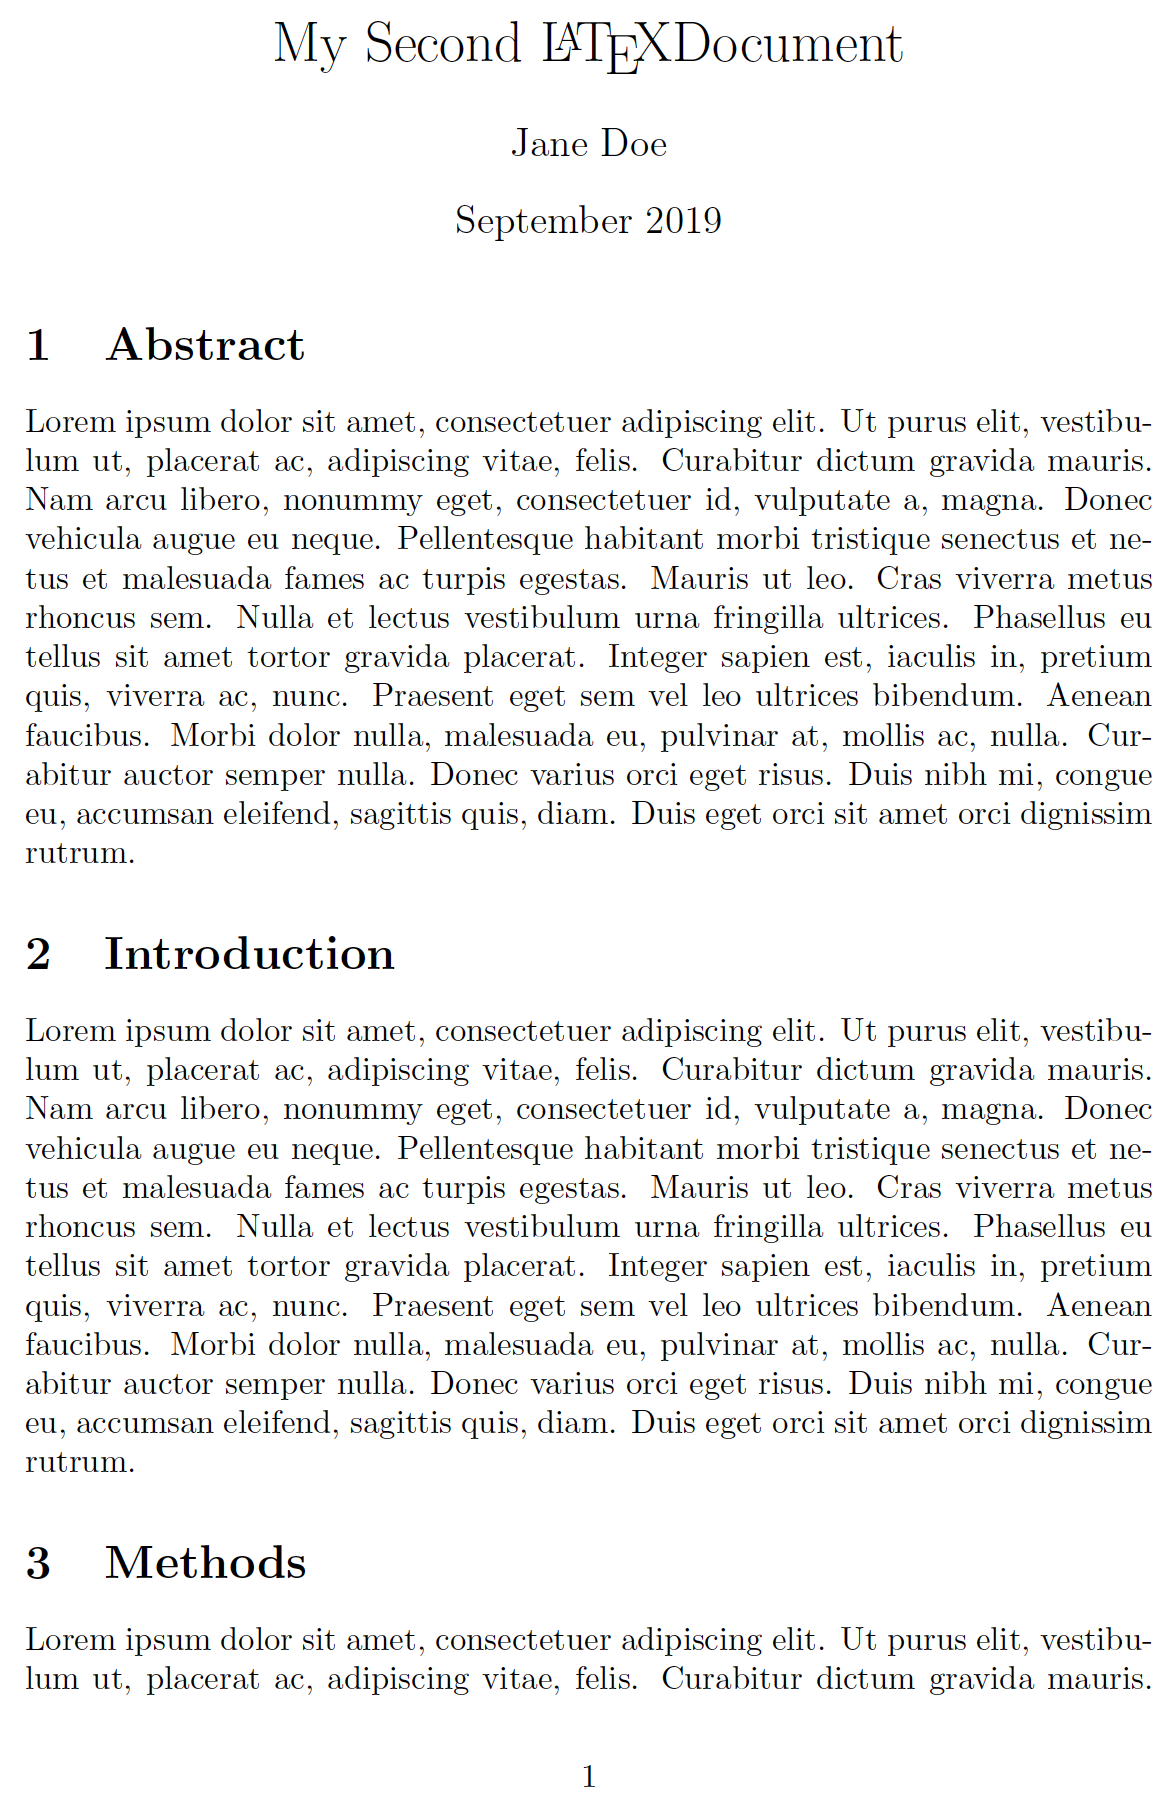
\includegraphics[width=.8\linewidth,keepaspectratio]{latex2a}
    \end{column}
    \begin{column}{0.5\textwidth}
      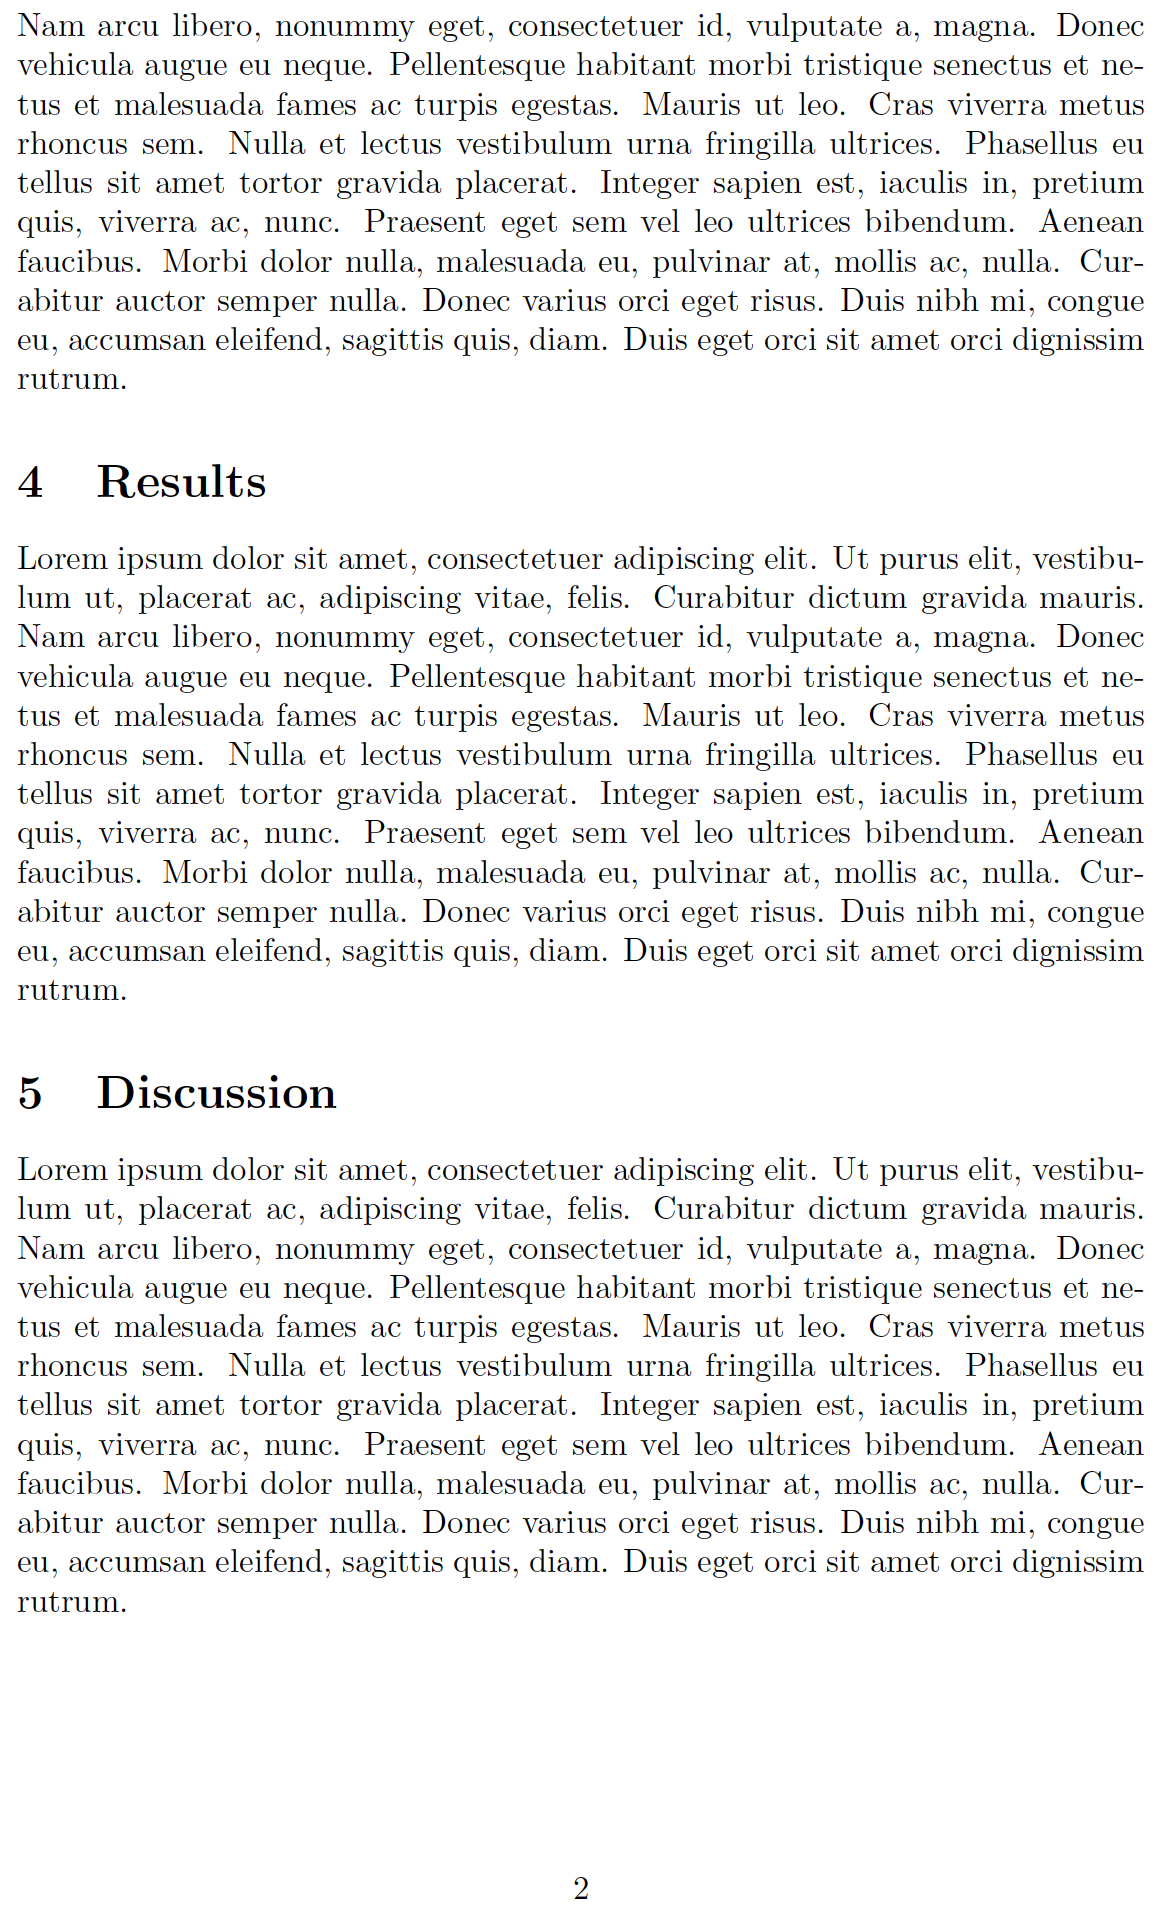
\includegraphics[width=.8\linewidth,keepaspectratio]{latex2b}
    \end{column}
  \end{columns}
\end{frame}

\begin{frame}{Exercise 1}
\footnotesize
\textbf{Using \LaTeX templates}
  \begin{itemize}
  \item Navigate to the folder: \texttt{/Rep-Res-Workshop/Presentation/LaTeXExercise/}
  \item Choose one of the templates from the journals Ecography, Journal of Animal Ecology (JAE), Journal of Wildlife Management (JWM), Proceedings of the National Academy of Science (PNAS), or Science.
  \item   Open the \texttt{.tex} file in the folder.
  \item Customize the template to include:
  \begin{itemize}
  \item Author names from a publication/project you are working on,
  \item Affiliations,
  \item Sections and sub-sections relevant for your work.
  \end{itemize}
  \item   Open the \texttt{.bib} file in the folder.
  \item Customize the .bib file to include:
  \begin{itemize}
  \item A reference from your field (go to Google Scholar, find an appropriate article, select the quotation marks below the article, and select "BibTeX" at the bottom of the pop-up window. Copy and past it into the .bib file)
  \end{itemize}
  \item Add the handle of the reference to the main .tex article using citep\{handle\} (with a backslash before citep).

\end{itemize}
\end{frame}

% ------------------------------------------------
\section{Using \texttt{knitr}}
% ------------------------------------------------

\begin{frame}[noframenumbering]
  \begin{center}
      \textsc{\textrm{Using}} \texttt{knitr}
  \end{center}
\end{frame}

\begin{frame}{What \texttt{knitr} Does}
  \begin{itemize}
  \item \texttt{knitr} ties together your presentation of results with the creation of those results
  \item Choose a mark-up code. We focus on \LaTeX in this workshop (an alternative is Markdown)
  \item Write document with mark-up code, with \texttt{R} chunks embedded in mark-up code.
  \item \texttt{knitr} converts \texttt{R} chunks to mark-up language (this would be tedious without \texttt{knitr})
  \item We can then compile final mark-up code using appropriate compiler
  \end{itemize}
\end{frame}

\begin{frame}
   \begin{center}
     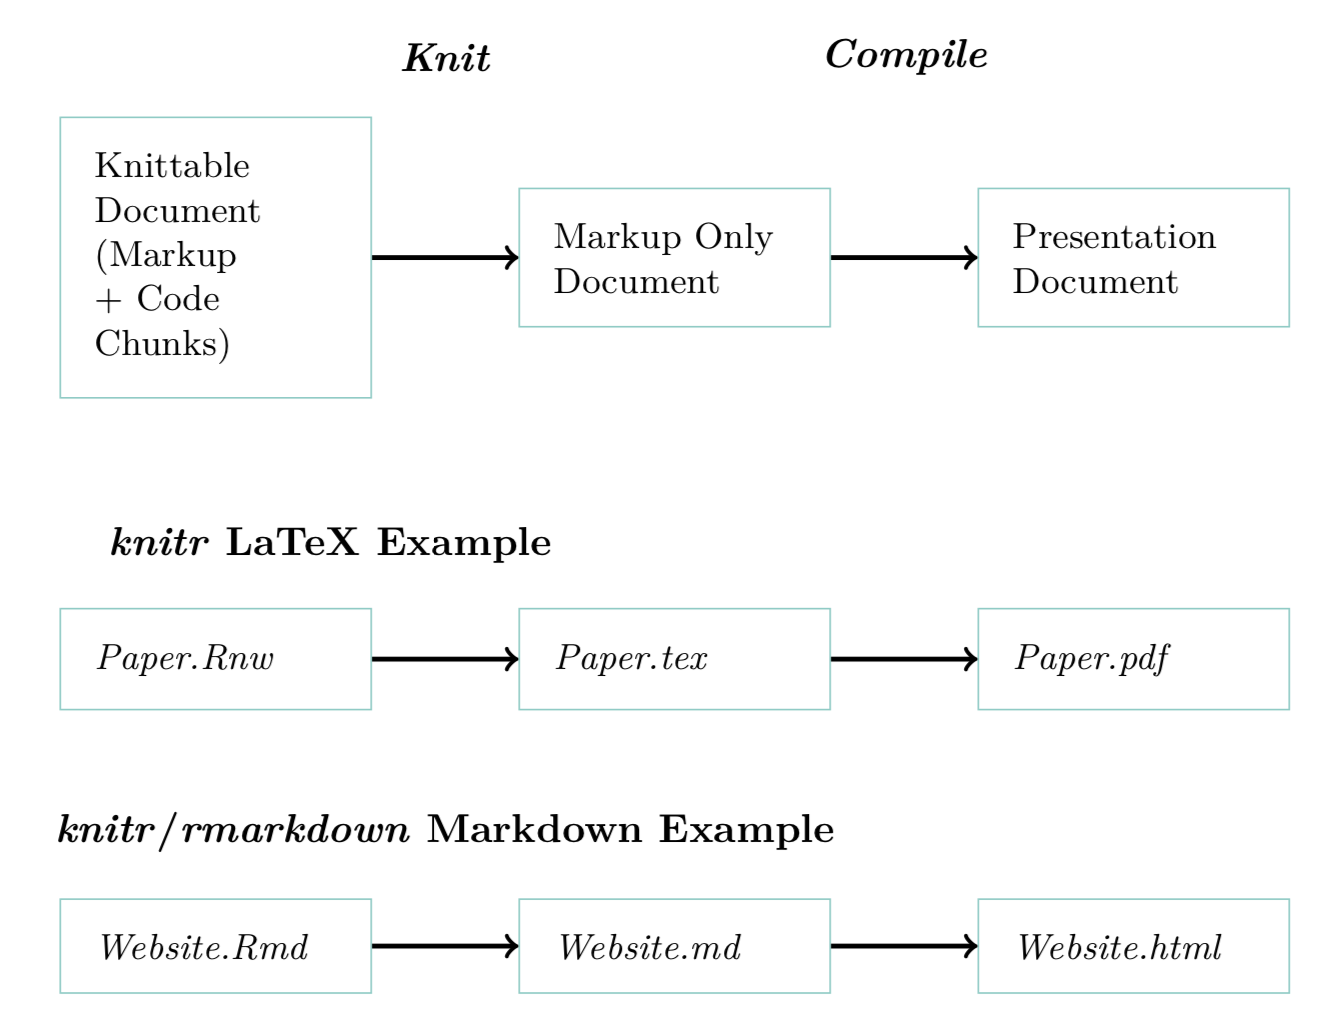
\includegraphics[width=.9\linewidth]{knitrprocess}
   \end{center}
 \end{frame}

\begin{frame}
   \begin{columns}
     \begin{column}{0.5\textwidth}
       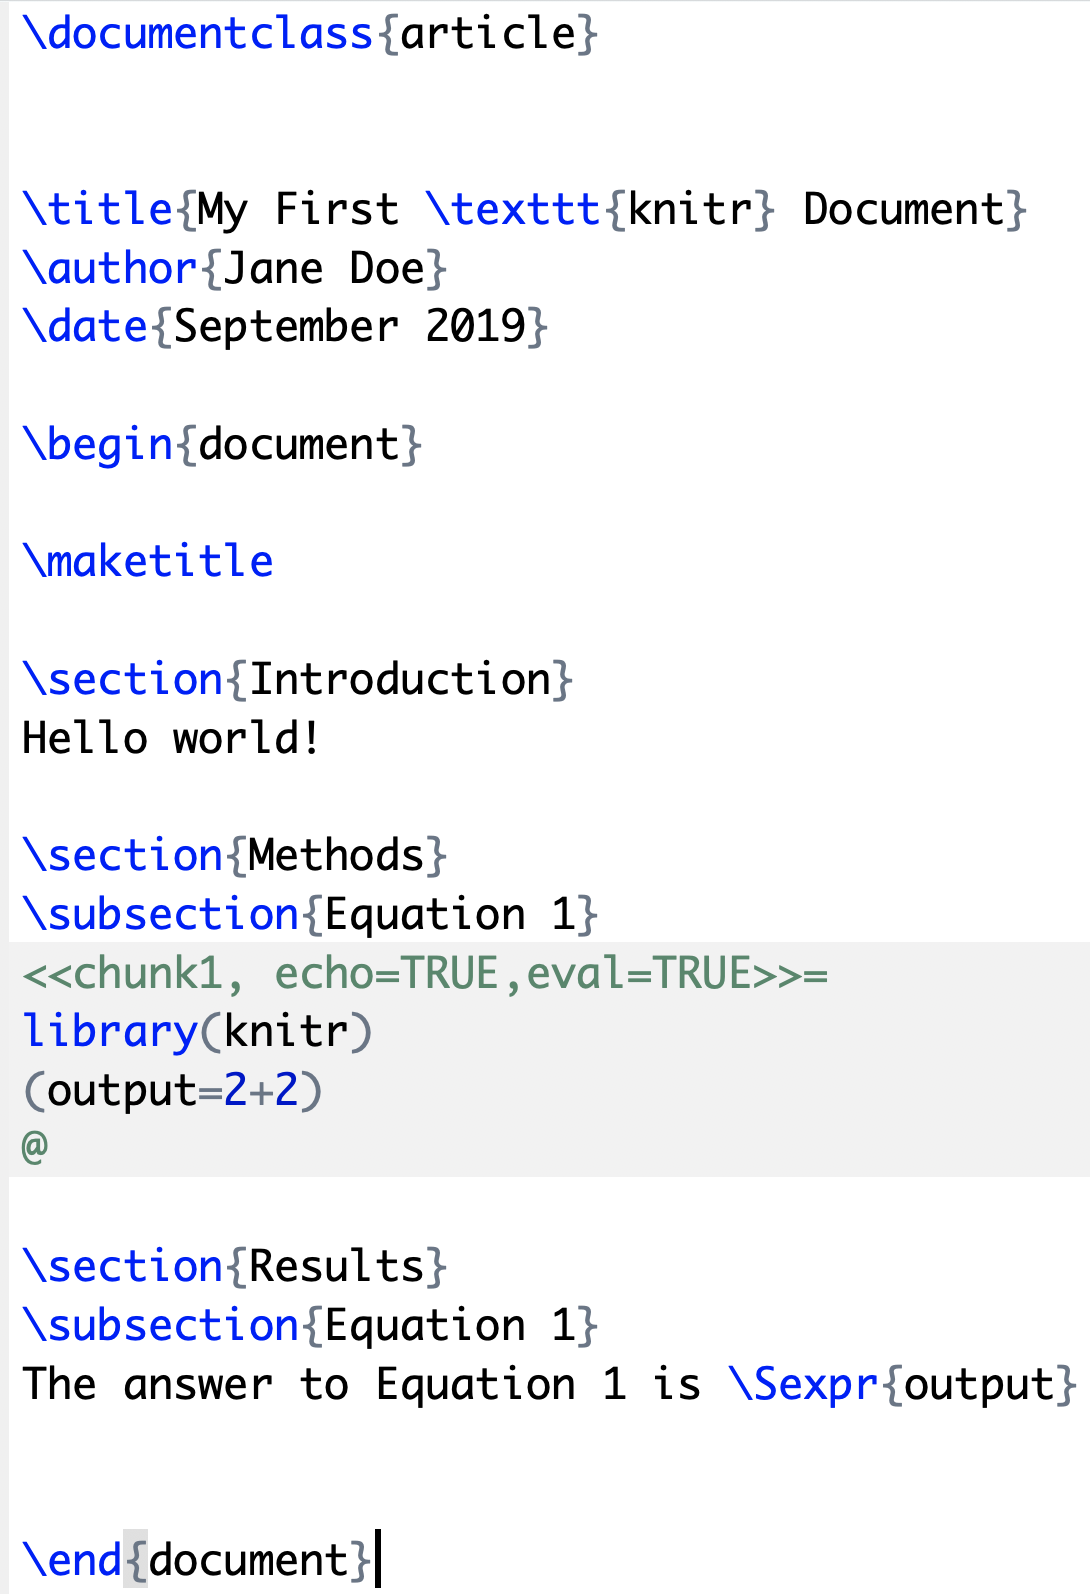
\includegraphics[width=.8\linewidth,keepaspectratio]{knitr1a}
      \end{column}
      \begin{column}{0.5\textwidth}
        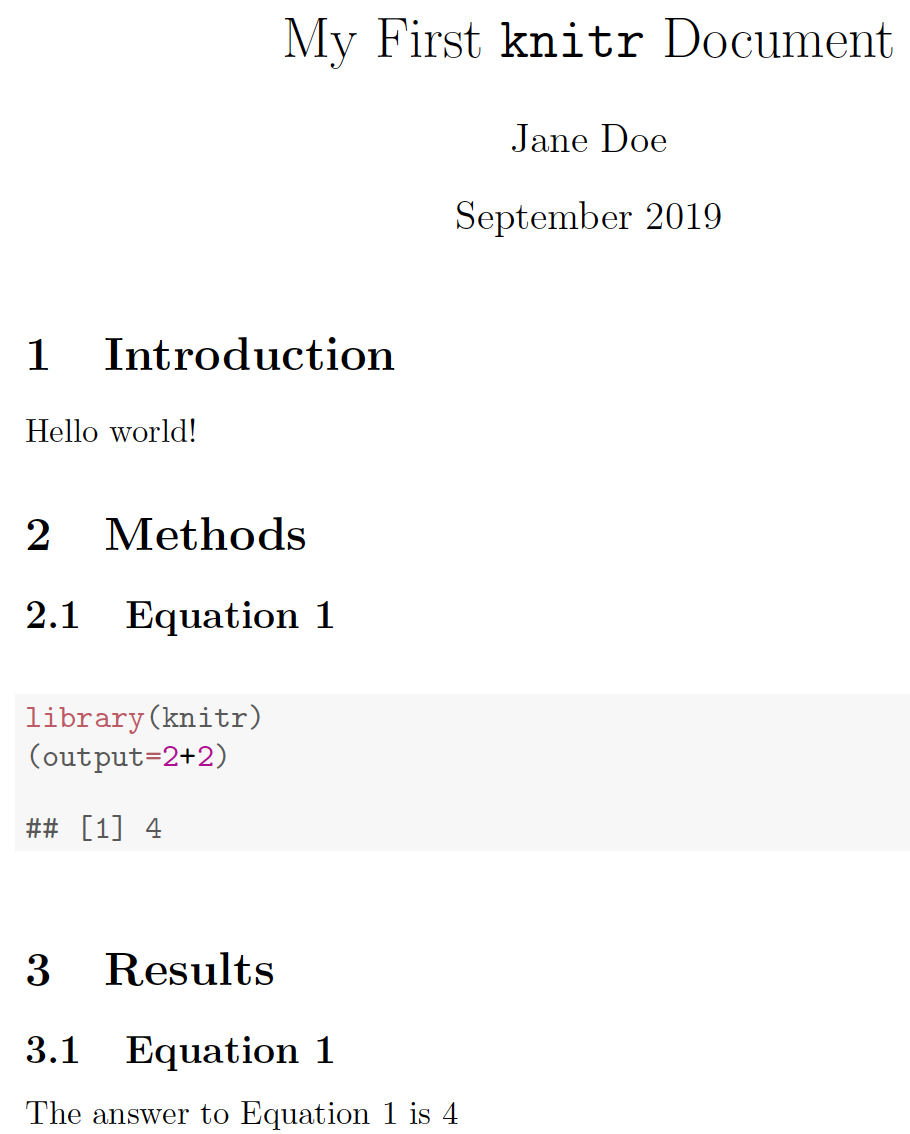
\includegraphics[width=.8\linewidth,keepaspectratio]{knitr1b}
      \end{column}
    \end{columns}
\end{frame}

\begin{frame}
   \begin{center}
     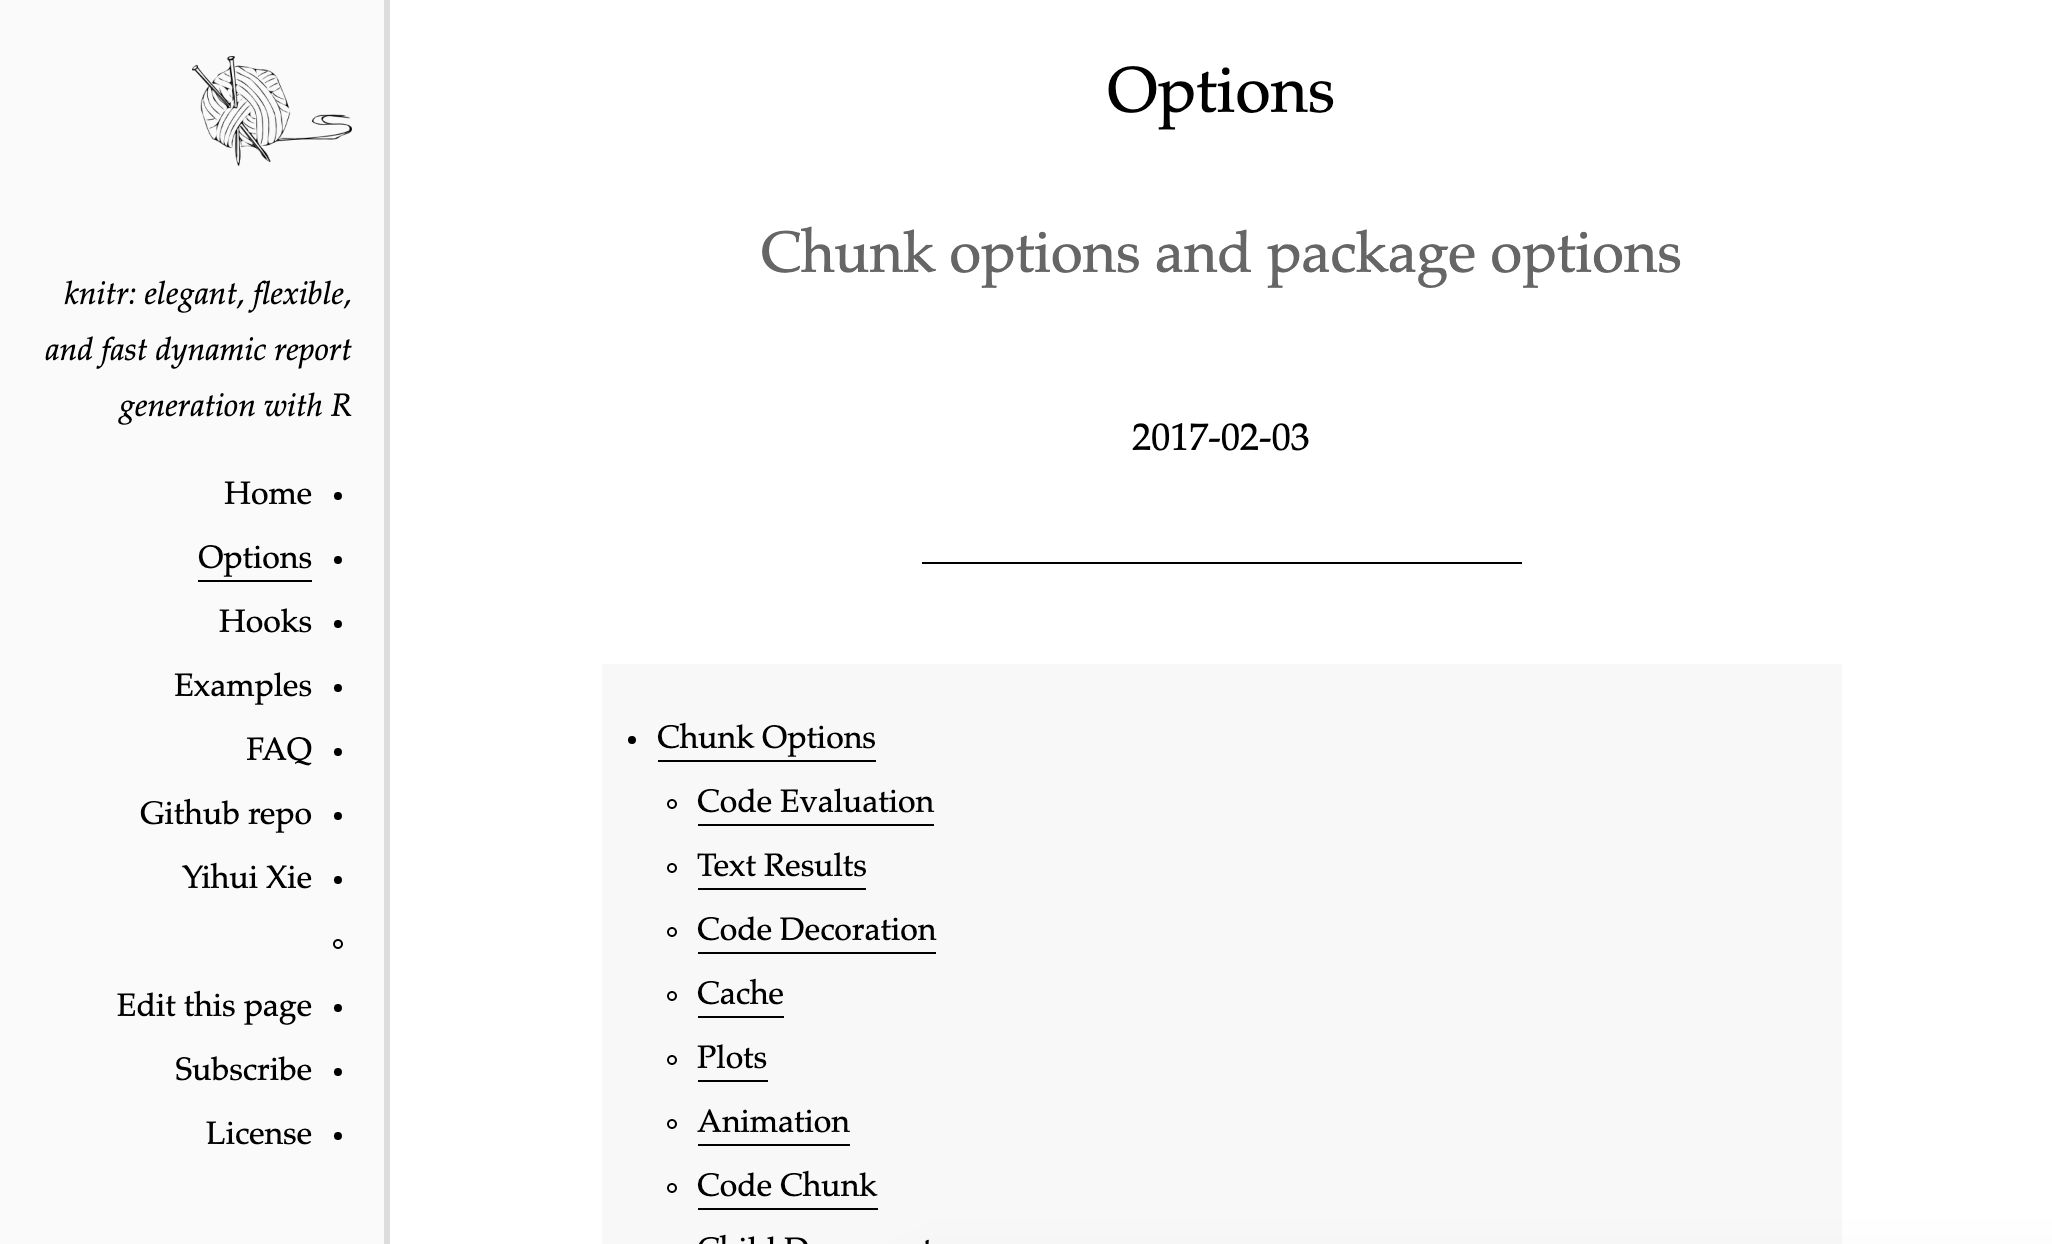
\includegraphics[width=.9\linewidth]{chunkoptions}
   \end{center}
\end{frame}


\begin{frame}{Second \texttt{knitr} document}
\end{frame}

\begin{frame}[t]{Exercise 2}
\textbf{Create an interactive \texttt{knitr} document that:}
\begin{itemize}
\item includes the analysis \texttt{MainAnalysis.R} within the \texttt{.Rnw} document,
\item replaces all static values (e.g., parameter estimates, figure and table numbers) with dynamic values from the incorporated analysis,
\item permits you to change the data in the analysis (i.e., remove Alaska), and automatically updates the parameter values.
\end{itemize}
\end{frame}

% ------------------------------------------------
\section{Organizing Workflow}
% ------------------------------------------------

\begin{frame}[noframenumbering]
  \begin{center}
      \textsc{\textrm{Organizing Workflow}}
  \end{center}
\end{frame}

\begin{frame}[t]{File Management}
\textbf{Careful file management is crucial for reproducible research}\\
\begin{itemize}
\item Explicitly tie your files together,
\item Have a plan to organize, store, and make your files available.
\end{itemize}
\end{frame}

\begin{frame}
   \begin{center}
     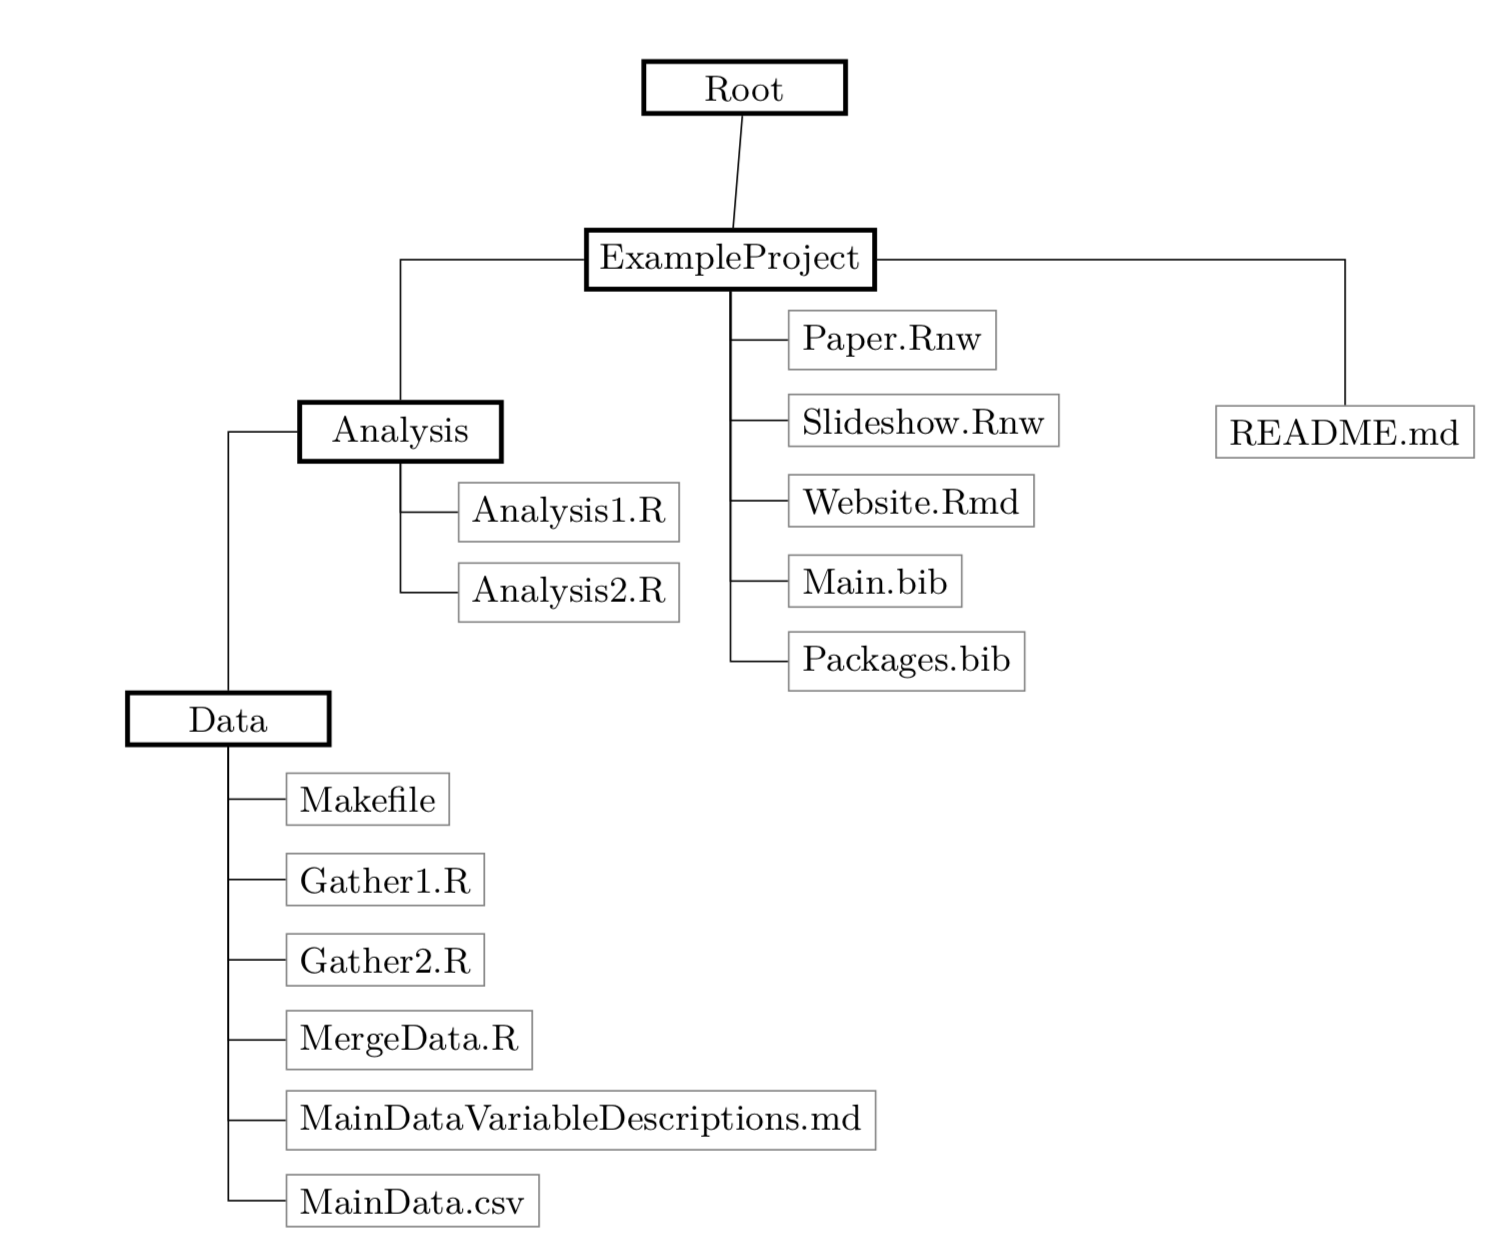
\includegraphics[width=.9\linewidth]{filemanagement}
   \end{center}
 \end{frame}

\begin{frame}[t]{File Management}
\begin{itemize}
\item If files are well organized and the way they are tied together is clear, replication will be much easier.
\item Permits easier changes to analyses.
\item Recycle work you have already done.
\end{itemize}
\end{frame}

\begin{frame}[t]{Is my research reproducible?}
\textbf{What formats are  your research documents stored in?}
\begin{itemize}
\item<2->.csv
\item<2->.txt
\item<2->.pdf
\item<2->.html
\item<2->.R or .RData
\end{itemize}
\only<3->{Yes, these are considered "reproducible"}
\begin{itemize}
\item<4->.doc or .docx
\item<4->.sas
\item<4->.xls or .xlsx
\item<4->any other proprietary file format
\end{itemize}
\only<5->{No, these are not considered "reproducible"}
\end{frame}

\begin{frame}[t]{Is my research reproducible?}
\textbf{Is your code linear?}
\begin{itemize}
\item<2->Clear environment often and at beginning of script
\item<2->Each program should focus on one main task or analysis
\item<2->Don't rely on manual commenting or uncommenting
\end{itemize}
\begin{center}
\only<2->{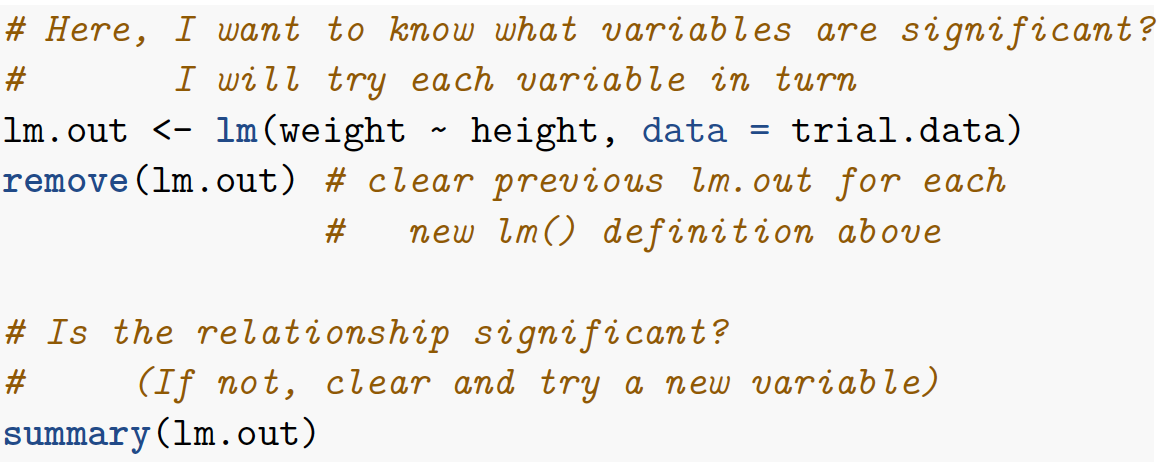
\includegraphics[width=0.9\linewidth]{nonlinear}}
\end{center}
\end{frame}

\begin{frame}[t]{Is my research reproducible?}
\textbf{Are your files easily shared with others?}
\begin{itemize}
\item<2->Organized directory structure
\item<2->Files relatively linked
\item<2->Well-documented \& commented
\item<2->Consistency in coding practices
\end{itemize}
\only<3->{"The point of having style guidelines is to have a common vocabulary of coding so people can concentrate on what you are saying, rahter than on how you are saying it." - Google's R Style Guide}
\end{frame}

\begin{frame}
\begin{center}

\includegraphics[width=\linewidth]{styleguide}
\end{center}
\end{frame}

\begin{frame}[t]{Is my research reproducible?}
\textbf{Do you treat your data as read only?}
\begin{itemize}
\item<2->Don't use Excel, etc., to manipulate raw data
\item<2->Use an \texttt{R} script for data processing
\item<2->Process data in one script, then save for loading into subsequent scripts
\item<2->When archiving, provide raw data and processing code, not just final tables
\end{itemize}
\end{frame}

\begin{frame}[t]{Additional Resources}
\begin{itemize}
\item https://swcarpentry.github.io/r-novice-gapminder/
02-project-intro/ (RStudio projects)
\item https://yihui.name/knitr/ (knitr help)
\item https://daringfireball.net/projects/markdown/basics (RMarkdown help)
\item https://rpubs.com/alobo/spintutorial (Roxygen)
\item http://eriqande.github.io/rep-res-web/ (online reproducible research course)
\item https://www.r-bloggers.com/rstudio-and-github/ (Github tutorial)
\end{itemize}
\end{frame}

\begin{frame}{Thank You!}
\begin{center}
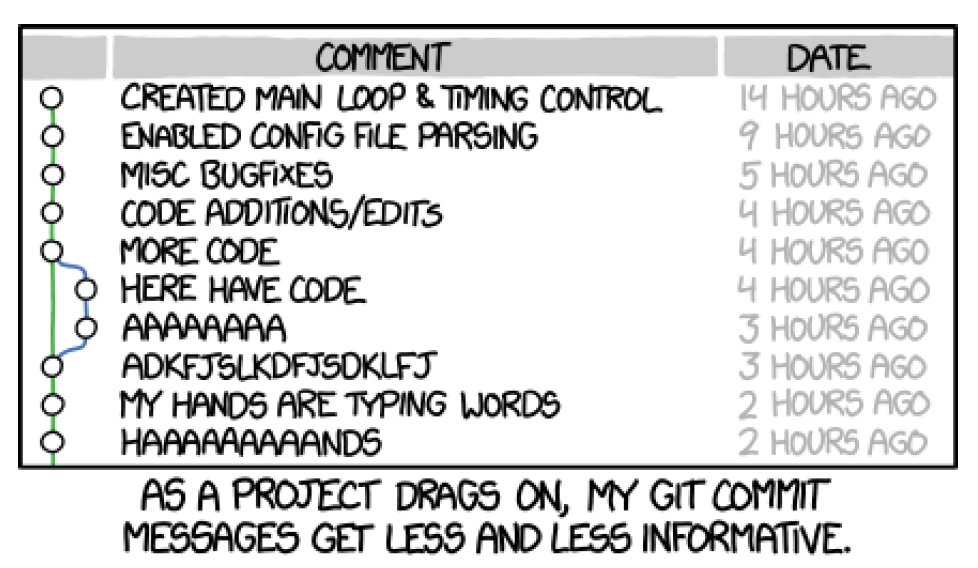
\includegraphics[width=0.6\linewidth]{gitcomments}
\end{center}
\end{frame}

\end{document}


